\documentclass[10pt,aspectratio=43,mathserif,table]{beamer} 
%  设置为 Beamer 文档类型,设置字体为 10pt,长宽比为16:9,数学字体为 serif 风格
\batchmode

\usepackage{fontspec}

\setmainfont{Harding Text Web Regular Regular.ttf}
\usepackage{diagbox} % 表头斜线分区
\usepackage{unicode-math}
\usefonttheme{serif}
\setmathrm{Harding Text Web Regular Regular.ttf} % 设置数学字体为 Times New Roman
\setmathfont{TeX Gyre Termes Math} % 如果您使用 XeLaTeX 或 LuaLaTeX 编译,可以使用其他数学字体
\setmathtt{Courier New} % 设置等宽字体为 Courier New
\setboldmathrm{Times New Roman}
\setmathfont{TeX Gyre Termes Math}[version=bold] % 设置粗体数学字体
\setmathfont{TeX Gyre Termes Math}[range={\mathit}]


\usetheme{Berlin} %主题
\setbeamertemplate{page number in head/foot}[pagenumber]
%\usecolortheme{sustech} %主题颜色

\usepackage[ruled,linesnumbered]{algorithm2e}

\usepackage{fancybox}
\usepackage{xcolor}
\usepackage{listings}

\usepackage{booktabs}
\usepackage{colortbl}

\newcommand{\Console}{Console}
\lstset{ %
	backgroundcolor=\color{white},   % choose the background color
	basicstyle=\footnotesize\rmfamily,     % size of fonts used for the code
	columns=fullflexible,
	breaklines=true,                 % automatic line breaking only at whitespace
	captionpos=b,                    % sets the caption-position to bottom
	tabsize=4,
	commentstyle=\color{mygreen},    % comment style
	escapeinside={\%*}{*)},          % if you want to add LaTeX within your code
	keywordstyle=\color{blue},       % keyword style
	stringstyle=\color{mymauve}\ttfamily,     % string literal style
	numbers=left, 
	%	frame=single,
	rulesepcolor=\color{red!20!green!20!blue!20},
	% identifierstyle=\color{red},
	language=c
}


\definecolor{mygreen}{rgb}{0,0.6,0}
\definecolor{mymauve}{rgb}{0.58,0,0.82}
\definecolor{mygray}{gray}{.9}
\definecolor{mypink}{rgb}{.99,.91,.95}
\definecolor{mycyan}{cmyk}{.3,0,0,0}

%题目,作者,学校,日期
\title{Paper Reading}
%\subtitle{\fontsize{9pt}{14pt}\textbf{跨临界分岔}}
\author{Speaker: Yichen Lu\quad \newline  \newline \quad }
\institute{\fontsize{8pt}{14pt}}
\date{\today}
\newcommand{\concept}{Paper Reading}

%学校Logo
%\pgfdeclareimage[height=0.5cm]{sustech-logo}{sustech-logo.pdf}
%\logo{\pgfuseimage{sustech-logo}\hspace*{0.3cm}}

\AtBeginSection[]
{
	\begin{frame}<beamer>
	\frametitle{\textbf{Contents}}
	\tableofcontents[currentsection]
\end{frame}
}
% \beamerdefaultoverlayspecification{<+->}
% -----------------------------------------------------------------------------
\begin{document}
% -----------------------------------------------------------------------------
% \frame{\titlepage}

\begin{frame}
    \begin{figure}
        \centering
        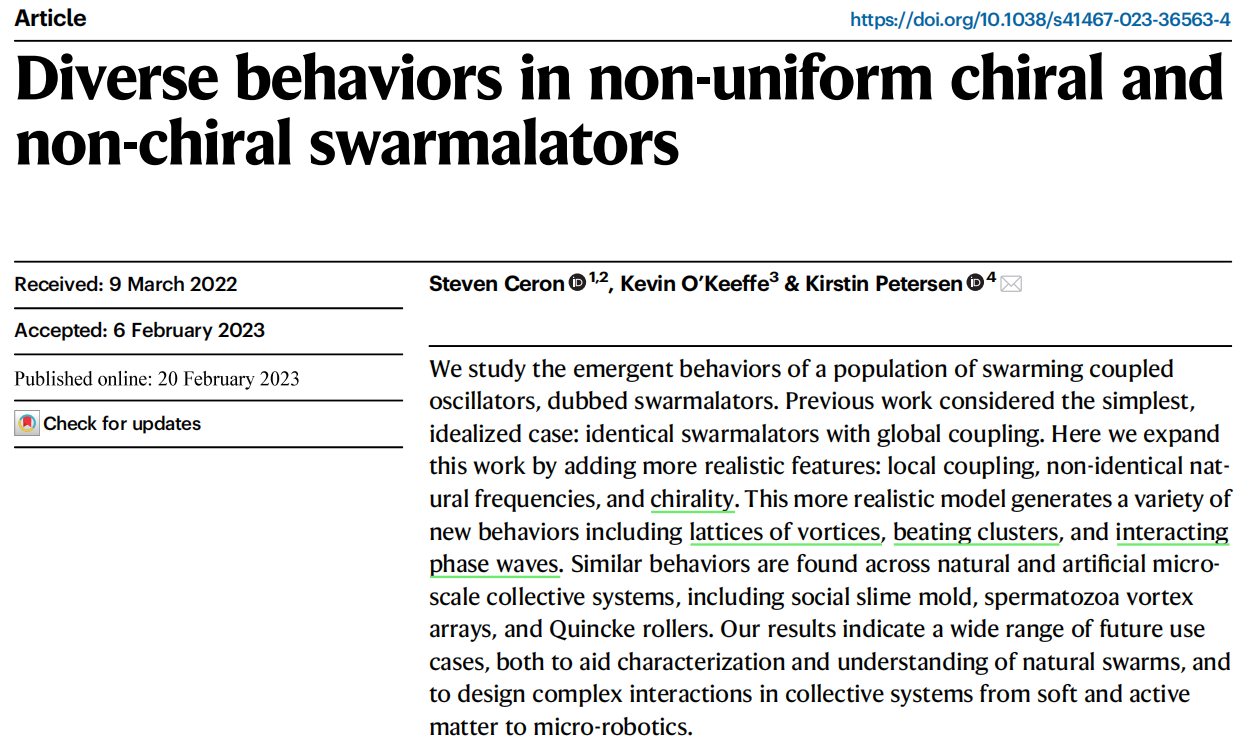
\includegraphics[width=\textwidth]{title.jpg}
    \end{figure}
    % 手性:swarmalators具有固定的圆形轨道,这个方向可以是顺时针也可以是逆时针
\end{frame}

\section{Non-chiral swarmalators}

\begin{frame}
    In the original model:
    % 在原来的模型中,是把所有粒子的自然速度的模都设为一个常数v_0,并且为0
        $$|\mathbf{v}_i|=v_0=0$$
    In this paper:
    % 在这篇paper中,作者做出了如下改进
        $$
        \mathbf{v}_i=c_i \mathbf{n}_i
        $$
    % 这么做的好处是速度与swarmalators的相位构成了一个直接映射,并且自然速度会像相位一样沿着圆形轨道的方向
        $$
        \begin{array}{c}
            c_i=\omega _iR_i\\
            \mathbf{n}_i=\left[ \begin{array}{c}
            \cos \left( \theta _i+\frac{\pi}{2} \right)\\
            \sin \left( \theta _i+\frac{\pi}{2} \right)\\
        \end{array} \right]\\
        \end{array}
        $$
    % 这里c_i依赖与自然频率omega_i和旋转半径R_i, n_i是一个单位向量,与相位角垂直,也就是说每个swarmalators的相位是它所在轨道上的角位置

\end{frame}

\begin{frame}
    New phase offset terms, $Q_{\dot{x}}$, $Q_{\dot{\theta}}$, which enable ‘frequency coupling’.
    % 文章还定义了新的相位偏移项,出发点是增加相反符号的自然品种的swarmalators之间的吸引力
    $$
    \begin{array}{c}
        Q_{\dot{x}}=\frac{\pi}{2}\left| \frac{\omega _j}{\left| \omega _j \right|}-\frac{\omega _i}{\left| \omega _i \right|} \right|\\
        Q_{\dot{\theta}}=\frac{\pi}{4}\left| \frac{\omega _j}{\left| \omega _j \right|}-\frac{\omega _i}{\left| \omega _i \right|} \right|\\
    \end{array}
    $$
    My understanding: 
    $$
    \begin{array}{c}
    Q_{\dot{x}}=\frac{\pi}{2}\left| \operatorname{sgn} \omega _j-\operatorname{sgn} \omega _i \right|=\begin{cases}
    \pi ,&		\operatorname{sgn} \omega _j\ne\operatorname{sgn} \omega _i\\
    0,&		\operatorname{sgn} \omega _j= \operatorname{sgn} \omega _i\\
    \end{cases}\\
    J\cos \left( \theta _j-\theta _i-Q_{\dot{x}} \right) =\begin{cases}
    -J\cos \left( \theta _j-\theta _i \right) ,&		Q_{\dot{x}}=\pi\\
    J\cos \left( \theta _j-\theta _i \right) ,&		Q_{\dot{x}}=0\\
    \end{cases}\\
    \end{array}
    $$
    
    
\end{frame}

\begin{frame}
    $$
    \dot{\mathbf{x}}_i=\mathbf{v}_i+\frac{1}{N}\sum_{j\ne i}^N{\left[ \frac{\mathbf{x}_j-\mathbf{x}_i}{\left| \mathbf{x}_j-\mathbf{x}_i \right|}\left( A+J\cos \left( \theta _j-\theta _i-Q_{\dot{x}} \right) \right) -B\frac{\mathbf{x}_j-\mathbf{x}_i}{\left| \mathbf{x}_j-\mathbf{x}_i \right|^2} \right]}
    $$

    $$
    J\cos \left( \theta _j-\theta _i-Q_{\dot{x}} \right) =\begin{cases}
        -J\cos \left( \theta _j-\theta _i \right) ,&		\operatorname{sgn} \omega _j\ne\operatorname{sgn} \omega _i\\
        J\cos \left( \theta _j-\theta _i \right) ,&		\operatorname{sgn} \omega _j= \operatorname{sgn} \omega _i\\
    \end{cases}
    $$
    \newline

    How can I ensure that $J\cos \left( \theta _j-\theta _i \right) > 0$, which means $\theta _j-\theta _i > \pi$ when $\operatorname{sgn} \omega _j\ne\operatorname{sgn} \omega _i$?
\end{frame}

\begin{frame}
    Model equations:
    $$
    \dot{\mathbf{x}}_i=\mathbf{v}_i+\frac{1}{N}\sum_{j\ne i}^N{\left[ \frac{\mathbf{x}_j-\mathbf{x}_i}{\left| \mathbf{x}_j-\mathbf{x}_i \right|}\left( A+J\cos \left( \theta _j-\theta _i-Q_{\dot{x}} \right) \right) -B\frac{\mathbf{x}_j-\mathbf{x}_i}{\left| \mathbf{x}_j-\mathbf{x}_i \right|^2} \right]}
    $$
    $$
    \dot{\theta}_i=\omega _i+\frac{K}{N}\sum_{j\ne i}^N{\frac{\sin \left( \theta _j-\theta _i-Q_{\dot{\theta}} \right)}{\left| \mathbf{x}_j-\mathbf{x}_i \right|}}
    $$
\end{frame}

\begin{frame}
    Several different cases of natural frequencies $\omega$ in this paper:
    \begin{figure}
        \centering
        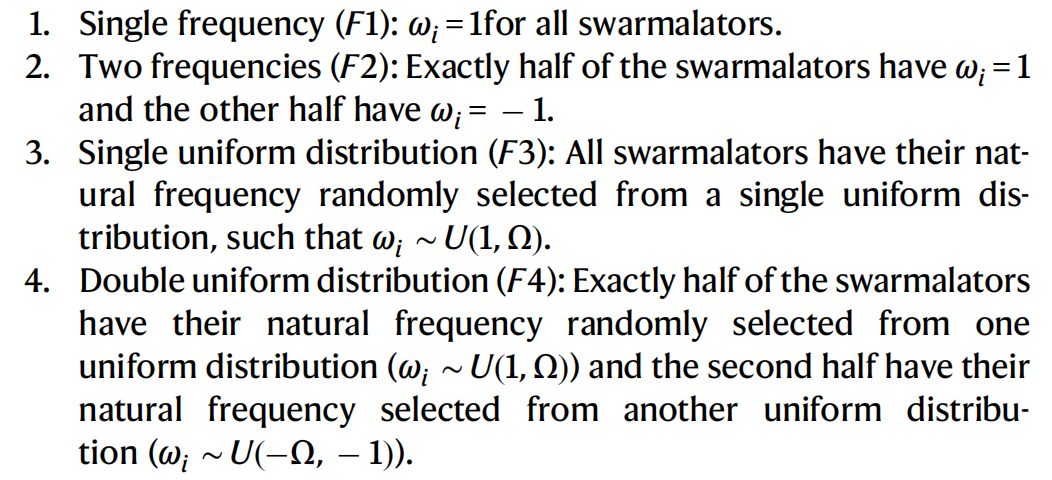
\includegraphics[width=\textwidth]{omega.jpg}
    \end{figure}
\end{frame}

\begin{frame}
    \begin{figure}
        \centering
        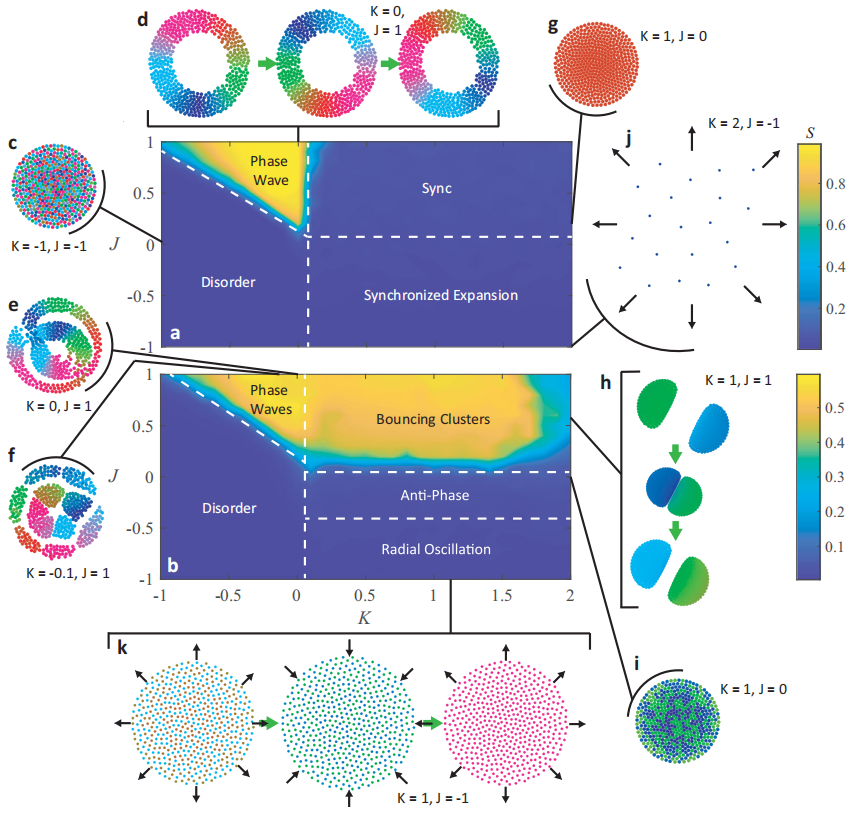
\includegraphics[width=0.75\textwidth]{fig2.jpg}
    \end{figure}
    % 图2e显示了两个相互作用的相位波,每一个都由相同自然频率的swarmalators组成;当两个环状结构形成的相位波绕着圆形边界移动时,会与相反的相位波相互作用。
    % 无论相位波是同心的还是互锁的,它们根据相位保持圆周排列,
    % 在K=-0/1. J=1的情况下,相同震动频率的swarmalators群体会形成分裂相位波,不同震动频率之间的相位波同心旋转,但方向相反。
    % 当不同的震动频率增加时,分裂出的相位波的数量也增加了,分裂出的相位波的数量和自然频率的数量是相关的。当有3个以上的自然频组时,组间的间距不清楚,旋转方向就不明确了。—— movie 2

    % 当自然频率分布为f2,也就是有2种时,会根据不同的频率形成两个群体,各自在内部形成并同步,并与频率相反的群体不同步。它们无法同步导致集体进入一个(bouncing cluster state)跳跃团簇状态,在这个状态下,每个群体在与另一个群体的吸引和排斥之间振荡,形成一种周期运动。这种振荡行为是由于群体具有相反的自然频率。当有2个以上的自然频率组时,他们的行为会更加复杂,而不是单轴的对称

    % 当K值很大,J=0时,具有自然频率分布𝐹2的集体形成环状结构并进入一种叫做(static anti-phase states)的状态,由于K值很大,他们在相位上的耦合很强,粒子在它们自己的自然频率组内同步,但又被相反组的相位抵消。由于J=0,使得相似相位的粒子之间在空间上没有吸引力,因此粒子在空间上均匀地分布在圆内。当K较小时,在相位上的耦合较小,此时相位波呈现出在径向方向上移动。

    % 当J<0时,相位相似的粒子会在空间上相互排斥,比如在K值比较大,粒子发生同步之后,由于都具有相同的相位,斥力会导致他们均匀碰撞。当有两种相反的自然频率时,粒子表现出的是在空间上径向的振荡状态,来自两个自然频率群的主体均匀分布在一个圆形地层中,并周期性地膨胀和收缩。这是因为当两组的相位差减小时,主体相互排斥,集体膨胀,但当相位差达到最大时,吸引力发生,群体收缩。
\end{frame}

\begin{frame}
    $$
    Z=\frac{1}{N}\sum_{j=1}^N{e^{i\left( \theta _j \right)}},\ \  \beta =\left| \frac{1}{n_{\omega}>0}\sum_{j=1}^{n_{\omega >0}}{\mathrm{x}_{\omega >0}}-\frac{1}{n_{\omega <0}}\sum_{j=1}^{n_{\omega <0}}{\mathrm{x}_{\omega <0}} \right|
    $$
    \begin{figure}
        \centering
        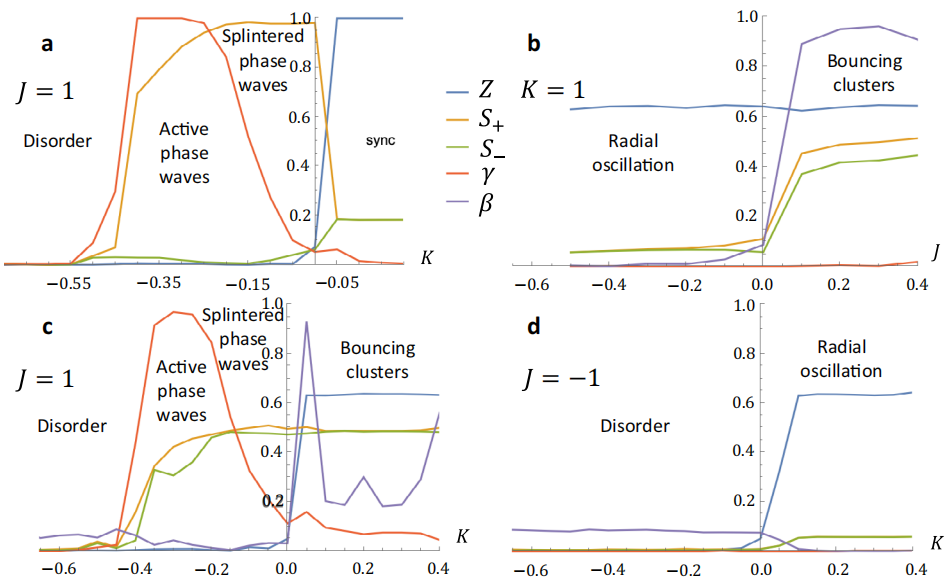
\includegraphics[width=0.8\textwidth]{fig3.jpg}
    \end{figure}
    % 下面是实验统计的一些序参量,
    % γ表示在暂态后,也就是稳定后在空间和相位上完成至少一个周期的swarmalators比例。
    % Z来自Kuramoto模型,表示相位同步的程度
    % β是自然频率为正和自然频率为负的swarmalators的平均位置的差值,也就是说,它是两个相位波之间的距离,所以当进入跳跃群体状态时,β会变大。
    % K是比较小的正值时,S保持在较高的取值,当K增加到很大后,有轻微的下降,这是因为当K增加时,相位波的数量也增加了,这使得相位波之间的相互作用增加,从而导致了S的下降。
\end{frame}

\section{Revolving swarmalators}

\begin{frame}{Revolving swarmalators}
    Revolving swarmalators’ motion and phase coupling behavior is defined when $c_i\ne 0$ for all agents and $Q_{\dot{x}}, Q_{\dot{\theta}}=0$
    $$
    \begin{cases}
        \dot{\mathbf{x}}_i=\mathbf{v}_i+\frac{1}{N}\sum_{j\ne i}^N{\left[ \frac{\mathbf{x}_j-\mathbf{x}_i}{\left| \mathbf{x}_j-\mathbf{x}_i \right|}\left( A+J\cos \left( \theta _j-\theta _i \right) \right) -B\frac{\mathbf{x}_j-\mathbf{x}_i}{\left| \mathbf{x}_j-\mathbf{x}_i \right|^2} \right]}\\
        \dot{\theta}_i=\omega _i+\frac{K}{N}\sum_{j\ne i}^N{\frac{\sin \left( \theta _j-\theta _i \right)}{\left| \mathbf{x}_j-\mathbf{x}_i \right|}}\\
        \mathbf{v}_i=\omega _i\left[ \begin{array}{c}
        \cos \left( \theta _i+\frac{\pi}{2} \right)\\
        \sin \left( \theta _i+\frac{\pi}{2} \right)\\
    \end{array} \right]\\
    \end{cases}
    $$

\end{frame}

\begin{frame}
    \begin{figure}
        \centering
        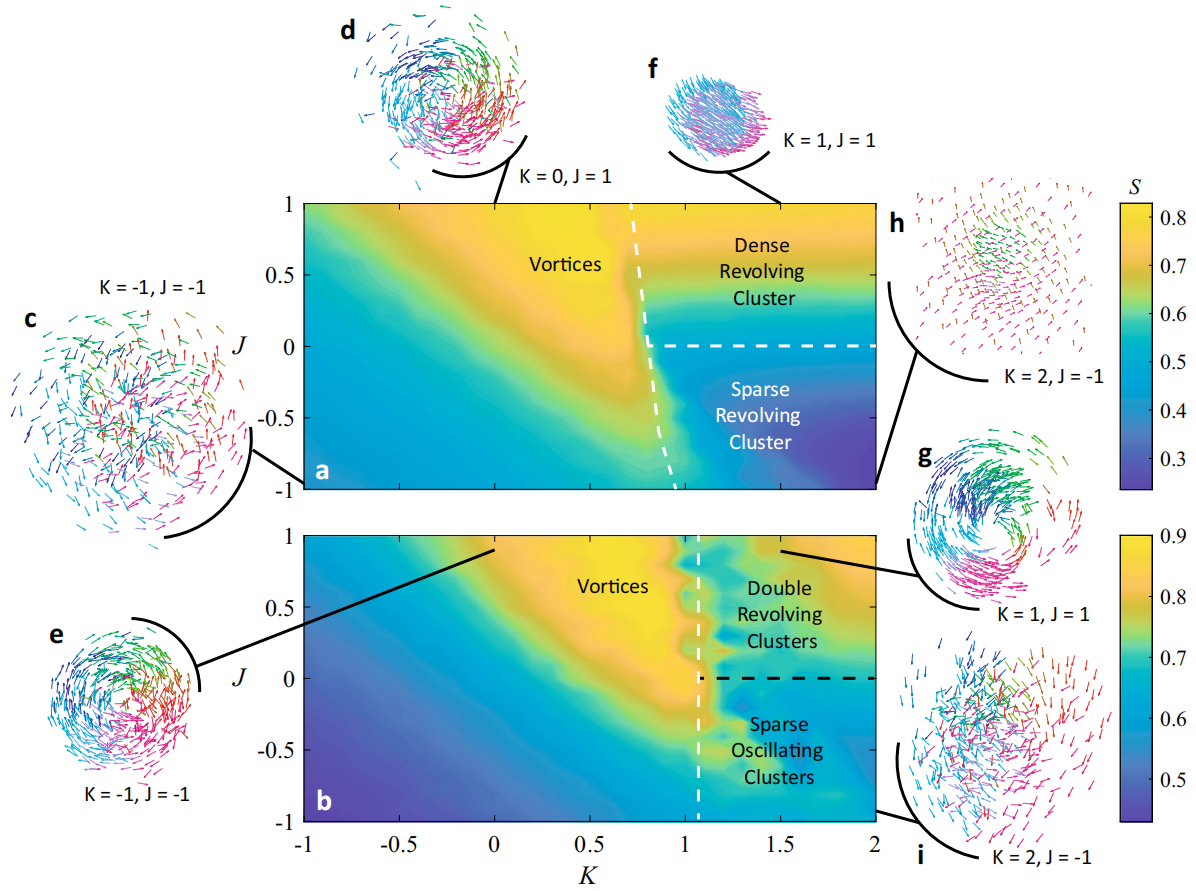
\includegraphics[width=0.9\textwidth]{fig4.png}
    \end{figure}
\end{frame}

\section{Frequency-coupled chiral swarmalators}

\begin{frame}{Frequency-coupled chiral swarmalators}
    $$
    \begin{cases}
        \dot{\mathbf{x}}_i=\mathbf{v}_i+\frac{1}{N}\sum_{j\ne i}^N{\left[ \frac{\mathbf{x}_j-\mathbf{x}_i}{\left| \mathbf{x}_j-\mathbf{x}_i \right|}\left( A+J\cos \left( \theta _j-\theta _i-Q_{\dot{x}} \right) \right) -B\frac{\mathbf{x}_j-\mathbf{x}_i}{\left| \mathbf{x}_j-\mathbf{x}_i \right|^2} \right]}\\
        \dot{\theta}_i=\omega _i+\frac{K}{N}\sum_{j\ne i}^N{\frac{\sin \left( \theta _j-\theta _i-Q_{\dot{\theta}} \right)}{\left| \mathbf{x}_j-\mathbf{x}_i \right|}}\\
        \mathbf{v}_i=\omega _i\left[ \begin{array}{c}
        \cos \left( \theta _i+\frac{\pi}{2} \right)\\
        \sin \left( \theta _i+\frac{\pi}{2} \right)\\
    \end{array} \right]\\
    \end{cases}
    $$
    $$
    \begin{array}{c}
        Q_{\dot{x}}=\frac{\pi}{2}\left| \frac{\omega _j}{\left| \omega _j \right|}-\frac{\omega _i}{\left| \omega _i \right|} \right|\\
        Q_{\dot{\theta}}=\frac{\pi}{4}\left| \frac{\omega _j}{\left| \omega _j \right|}-\frac{\omega _i}{\left| \omega _i \right|} \right|\\
    \end{array}
    $$
\end{frame}

\begin{frame}
    \begin{figure}
        \centering
        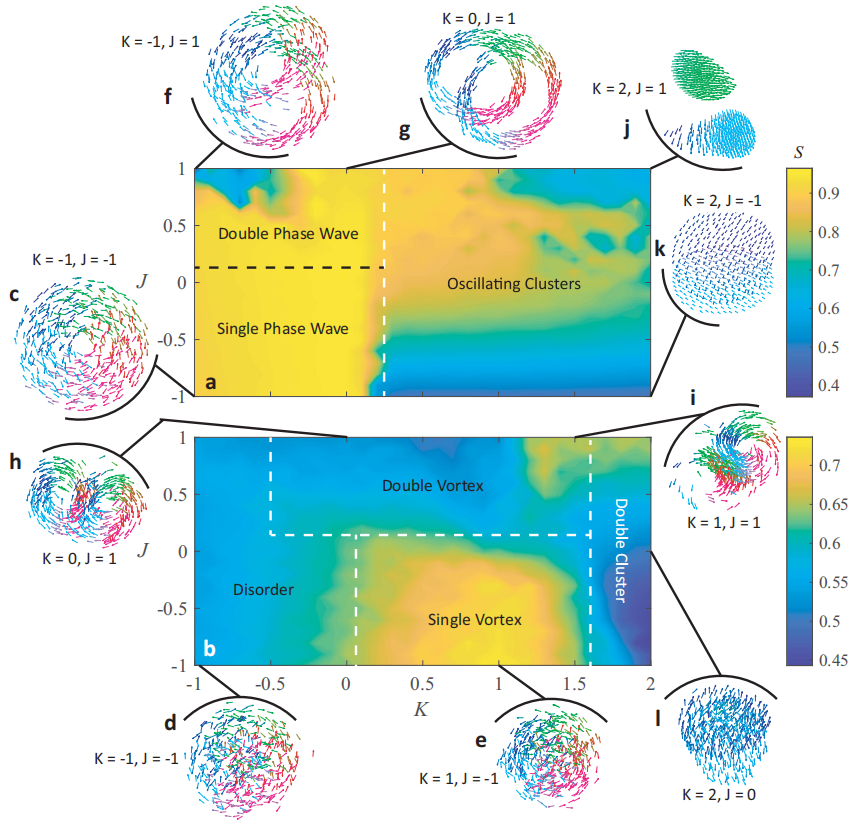
\includegraphics[width=0.75\textwidth]{fig6.png}
    \end{figure}
    % Q项目的加入增强了相反符号频率粒子之间的斥力,当J较大时,原来同心的轨道现在变成互锁的. 
\end{frame}


% -----------------------------------------------------------------------------
\end{document}

